\documentclass[a4 paper]{article}
\usepackage[inner=2.0cm,outer=2.0cm,top=2.5cm,bottom=2.5cm]{geometry}
\usepackage{setspace}
\usepackage[rgb]{xcolor}
\usepackage{verbatim}
\usepackage{subcaption}
\usepackage{amsgen,amsmath,amstext,amsbsy,amsopn,tikz,amssymb}
\usepackage{fancyhdr}
\usepackage[colorlinks=true, urlcolor=blue,  linkcolor=blue, citecolor=blue]{hyperref}
\usepackage[colorinlistoftodos]{todonotes}
\usepackage{rotating}
\usepackage{booktabs}
\newcommand{\ra}[1]{\renewcommand{\arraystretch}{#1}}

\newtheorem{thm}{Theorem}[section]
\newtheorem{prop}[thm]{Proposition}
\newtheorem{lem}[thm]{Lemma}
\newtheorem{cor}[thm]{Corollary}
\newtheorem{defn}[thm]{Definition}
\newtheorem{rem}[thm]{Remark}
\numberwithin{equation}{section}

\newcommand{\homework}[6]{
   \pagestyle{myheadings}
   \thispagestyle{plain}
   \newpage
   \setcounter{page}{1}
   \noindent
   \begin{center}
   \framebox{
      \vbox{\vspace{2mm}
    \hbox to 6.28in { {\bf CSE 211:~Discrete Mathematics \hfill {\small (#2)}} }
       \vspace{6mm}
       \hbox to 6.28in { {\Large \hfill #1  \hfill} }
       \vspace{6mm}
       \hbox to 6.28in { {\it Instructor: {\rm #3} \hfill  {\rm #5} \hfill  {\rm #6}} \hfill}
       \hbox to 6.28in { {\it Assistant: #4  \hfill #6}}
      \vspace{2mm}}
   }
   \end{center}
   \markboth{#5 -- #1}{#5 -- #1}
   \vspace*{4mm}
}

\newcommand{\problem}[2]{~\\\fbox{\textbf{Problem #1}}\hfill (#2 points)\newline\newline}
\newcommand{\subproblem}[1]{~\newline\textbf{(#1)}}
\newcommand{\D}{\mathcal{D}}
\newcommand{\Hy}{\mathcal{H}}
\newcommand{\VS}{\textrm{VS}}
\newcommand{\solution}{~\newline\textbf{\textit{(Solution)}} }

\newcommand{\bbF}{\mathbb{F}}
\newcommand{\bbX}{\mathbb{X}}
\newcommand{\bI}{\mathbf{I}}
\newcommand{\bX}{\mathbf{X}}
\newcommand{\bY}{\mathbf{Y}}
\newcommand{\bepsilon}{\boldsymbol{\epsilon}}
\newcommand{\balpha}{\boldsymbol{\alpha}}
\newcommand{\bbeta}{\boldsymbol{\beta}}
\newcommand{\0}{\mathbf{0}}


\begin{document}
\homework{Homework \#2}{Due: 07/12/20}{Dr. Zafeirakis Zafeirakopoulos}{Gizem S\"ung\"u}{}{}
\textbf{Course Policy}: Read all the instructions below carefully before you start working on the assignment, and before you make a submission.
\begin{itemize}
\item It is not a group homework. Do not share your answers to anyone in any circumstance. Any cheating means at least -100 for both sides. 
\item Do not take any information from Internet.
\item No late homework will be accepted. 
\item For any questions about the homework, send an email to gizemsungu@gtu.edu.tr
\item The homeworks (both latex and pdf files in a zip file) will be
submitted into the course page of Moodle.
\item The latex, pdf and zip files of the homeworks should be saved as
"Name\_Surname\_StudentId".$\{$tex, pdf, zip$\}$.
\item If the answers of the homeworks have only calculations without any formula or any explanation -when needed- will get zero.
\item Writing the homeworks on Latex is strongly suggested. However, hand-written paper is still accepted $\textbf{IFF}$ hand writing of the student is clear and understandable to read, and the paper is well-organized. Otherwise, the assistant cannot grade the student's homework.
\end{itemize}

\problem{1: Relations}{15}
Draw the Hasse diagram for the “greater than or equal to” relation on $\{$0, 1, 2, 3, 4, 5$\}$. In order to draw the diagram, you can choose one of the following options:

\begin{itemize}
	\item You can use an online drawing tool such as https://app.diagrams.net/.
	\item You can draw the diagram by hand, take a picture of it to put on Latex as a figure.
	\item Word Office, Libre Office are also options to use them as drawing tools. 
\end{itemize}
\solution 

\newline 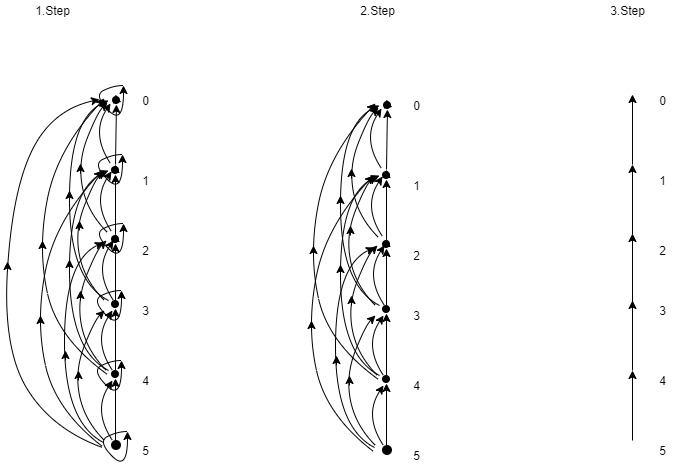
\includegraphics[width=120mm]{hasse.jpg}
\newline
\newline A=$\{(0 \prec 0),(0 \prec 1),(0 \prec 2),(0 \prec 3),(0 \prec 4),(0 \prec 5)(1 \prec 1),(1 \prec 2),(1 \prec 3),(1 \prec 4),(1 \prec 5),(2 \prec 2),(2 \prec 3),(2 \prec 4),(2 \prec 5),(3 \prec 3),(3 \prec 4),(3 \prec 5),(4 \preceq 4),(4 \prec 5),(5 \prec 5)\}$
\newline
\newline
\newline 1.Step:We first draw the directed graph to the relation R.The graph needs to contain loops at every vertex, because elements are always greater than or equal to itself.
\newline
\newline 
\newline A=$\{(0 \prec 1),(0 \prec 2),(0 \prec 3),(0 \prec 4),(0 \prec 5),(1 \prec 2),(1 \prec 3),(1 \prec 4),(1 \prec 5),(2 \prec 3),(2 \prec 4),(2 \prec 5),(3 \prec 4),(3 \prec 5),(4 \prec 5)\}$
\newline
\newline
\newline 2.Step: We remove all loops form the diagram.Because loops are always present in a reflexive, we don't have to shown them.We remove any arrows on the directed edges.
\newline
\newline A=$\{(0 \prec 1),(1 \prec 2),(2 \prec 3),(3 \prec 4),(4 \prec 5)\}$
\newline
\newline 3.Step: Finally, we remove all loops from the diagram because R is a partial order and since loops are always present in a partial order(reflexive),we do not have to shown them.
\newpage
\problem{2: Relations}{15}
Answer these questions for the poset ($\{\{$1$\}$, $\{$2$\}$, $\{$4$\}$, $\{$1, 2$\}$, $\{$1, 4$\}$, $\{$2, 4$\}$, $\{$3, 4$\}$, $\{$1, 3, 4$\}$, $\{$2, 3, 4$\}\}$, $\subseteq$).
\subproblem{a} Find the maximal elements.
\solution $\{\{$1,2$\}$, $\{$2,3,4$\},\{$1,3,4$\}\}$
\subproblem{b} Find the minimal elements.
\solution $\{\{$1$\}$, $\{$2$\},\{$4$\}\}$
\subproblem{c} Is there a greatest element?
\solution Does not exist
\subproblem{d} Find all upper bounds of $\{\{$2$\}$, $\{$4$\}\}$.
\solution  $\{\{$2,4$\},\{$2,3,4$\}\}$
\subproblem{e} Find the least upper bound of $\{\{$2$\}$, $\{$4$\}\}$, if it exists.
\solution $\{2,4\}$
\subproblem{f} Find all lower bounds of $\{\{$1, 3, 4$\}$, $\{$2, 3, 4$\}\}$.
\solution $\{\{$4$\},\{$3,4$\}\}$
\subproblem{h} Find the greatest lower bound of $\{\{$1, 3, 4$\}$, $\{$2, 3, 4$\}\}$,
if it exists.
\solution $\{3,4\}$
\newline
\newline
\newline
\newline
\newline 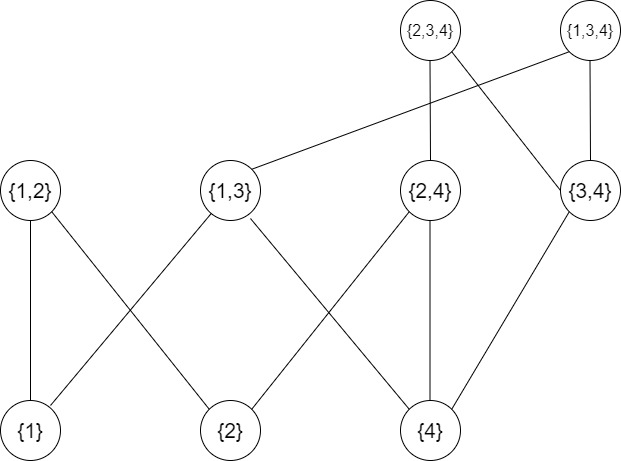
\includegraphics[width=120mm]{poset.jpg}
\newpage
\problem{3: Relations}{70}
Remember that a relation $R$ on a set $A$ can have the properties reflexive, symmetric, anti-symmetric and transitive.

\begin{itemize}
	\item $\textbf{Reflexive: }$ R is reflexive if (a, a) $\in$ $R$, $\forall$ a $\in$ A.
	\item $\textbf{Symmetric: }$ R is symmetric if (b, a) $\in$ R whenever (a, b) $\in$ R, $\forall$ a, b $\in$ A.
	\item $\textbf{Anti-symmetric: }$ R is antisymmetric if $\forall$ a, b $\in$ A, (a, b) $\in$ R and (b, a) $\in$ R implies that a = b.
	\item $\textbf{Transitive: }$ R is transitive if $\forall$ a, b, c $\in$ A, (a, b) $\in$ R and (b, c) $\in$ R implies that (a, c) $\in$ R.
\end{itemize}
For the details about the properties, please check the 4th lecture slide on Moodle. \\

As we solved the problem 3 in PS4 document - which is available on Moodle - in the problem session, we can determine any given relation if it is reflexive, symmetric, anti-symmetric, and transitive.\\

Write an algorithm to determine if a given relation $R$ is reflexive, symmetric, anti-symmetric, and transitive. Your code should meet the following requirements, standards and tasks.

\begin{itemize}
	\item Read the relations in the text file "input.txt".
	\item Let $R$ be a relation on a set $A$ where $\exists a,b \in A, (a,b) \in R$. Each relation $R$ is represented with 3 lines in the file:
	\begin{itemize}
		\item [1.] The first line says how many relations in $R$.
		\item[2.] The second line gives the elements of the set $A$.
		\item[3.] The following lines gives each relation in $R$.
	\end{itemize}
	\item After determining each relation in input.txt whether it is reflexive, symmetric, anti-symmetric and transitive with your algorithm, write its result to the file which is called "output.txt" with the following format.
	\item output.txt:
	\begin{itemize}
		\item[1.] Start a new line with "n" which indicates a new relation.
		\item[2.] The set of $R$
		\item[3.] Reflexive: Yes or No, explain the reason if No (e.g. "(a, a) is not found").
		\item[4.] Symmetric: Yes or No, explain the reason if No (e.g. "(b, a) is not found whereas (a, b) is found.")
		\item[5.] Antisymmetric: Yes or No, explain the reason if No (e.g. "(b, a) and (a, b) are found.")
		\item[6.] Transitive: Yes or No, explain the reason if No (e.g. "(a, c) is not found whereas (a, b) and (b, c) are found.")
	\end{itemize}
	\item An example of the output format is given in "exampleoutput.txt". The file has the result of the first relation in "input.txt".
	\item When explaining why a property does not exist in the relation, one reason is enough to explain if there are more. For example, in "exampleoutput.txt", the relation is not symmetric because (b, a) and (e, a) are not found. Detecting one of them is enough to explain the reason.
	\item $\textbf{Bonus (20 points): }$ If you can explain why a property exists in the relation, it brings you bonus of 20 points.
	\item Your code is responsible to provide exception and error handling. The input file may be given with a wrong information, then your code must be prepared to detect them. For instance, "The element b of the relation (1, b) is not found in the set A = $\{1, 2, 3, 4\}$.".
	\item You can implement your algorithm in Python, Java, C or C++.
	\item $\textbf{Important: }$ Put comments almost for each line of your code to describe what the line is going to do. 
	\item You should put your source code file (file name is problem1.$\{.c, .java, .py, .cpp\}$) and output.txt into your homework zip file (check Course Policy).
\end{itemize}



\end{document} 
